\documentclass{standalone}
\usepackage{tikz}
\usetikzlibrary{patterns}
\usetikzlibrary{positioning}
\usetikzlibrary{patterns, positioning}
\usetikzlibrary{shapes.misc}
\usepackage[outline]{contour}
\contourlength{1.5pt} 


\begin{document}
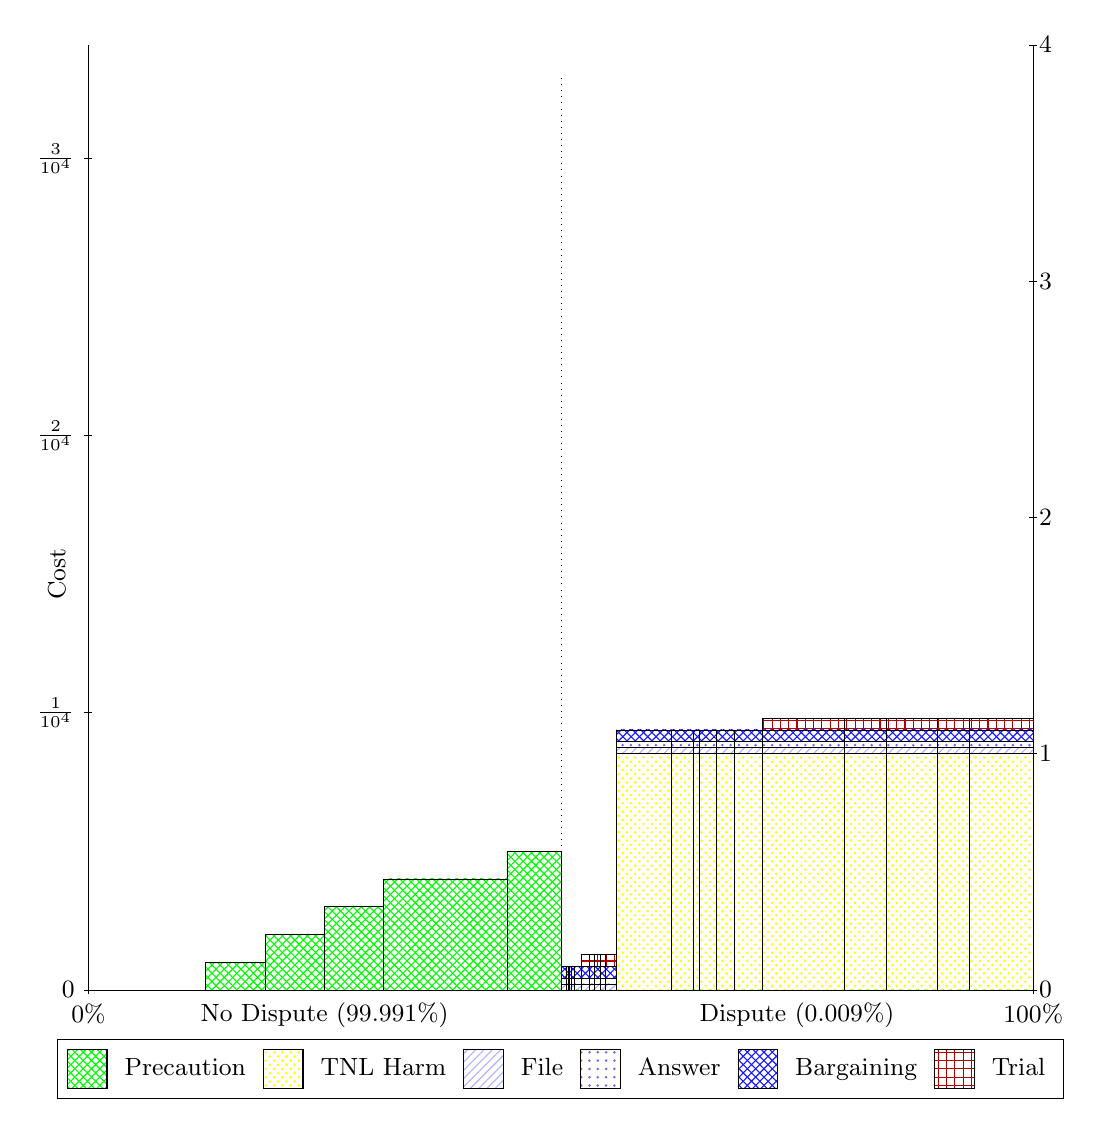
\begin{tikzpicture}
\draw[pattern=crosshatch, pattern color=green,draw=black,very thin] (2.9856,2.5) rectangle (3.7488,2.8519);
\draw[pattern=crosshatch, pattern color=green,draw=black,very thin] (3.7488,2.5) rectangle (4.4999,3.2037);
\draw[pattern=crosshatch, pattern color=green,draw=black,very thin] (4.4999,2.5) rectangle (5.2511,3.5556);
\draw[pattern=crosshatch, pattern color=green,draw=black,very thin] (5.2511,2.5) rectangle (6.8167,3.9074);
\draw[pattern=crosshatch, pattern color=green,draw=black,very thin] (6.8167,2.5) rectangle (7.5,4.2593);
\draw[pattern=north east lines, pattern color=blue!30,draw=black,very thin] (7.5,2.5) rectangle (7.57,2.575);
\draw[pattern=dots,  pattern color=blue!60,draw=black,very thin] (7.5,2.575) rectangle (7.57,2.65);
\draw[pattern=crosshatch,      pattern color=blue!90,draw=black,very thin] (7.5,2.65) rectangle (7.57,2.8);
\draw[pattern=crosshatch, pattern color=green,draw=black,very thin] (7.57,2.5) rectangle (7.6004,2.5);
\draw[pattern=north east lines, pattern color=blue!30,draw=black,very thin] (7.57,2.5) rectangle (7.6004,2.575);
\draw[pattern=dots,  pattern color=blue!60,draw=black,very thin] (7.57,2.575) rectangle (7.6004,2.65);
\draw[pattern=crosshatch,      pattern color=blue!90,draw=black,very thin] (7.57,2.65) rectangle (7.6004,2.8);
\draw[pattern=crosshatch, pattern color=green,draw=black,very thin] (7.6004,2.5) rectangle (7.6092,2.5001);
\draw[pattern=north east lines, pattern color=blue!30,draw=black,very thin] (7.6004,2.5001) rectangle (7.6092,2.5751);
\draw[pattern=dots,  pattern color=blue!60,draw=black,very thin] (7.6004,2.5751) rectangle (7.6092,2.6501);
\draw[pattern=crosshatch,      pattern color=blue!90,draw=black,very thin] (7.6004,2.6501) rectangle (7.6092,2.8001);
\draw[pattern=crosshatch, pattern color=green,draw=black,very thin] (7.6092,2.5) rectangle (7.6386,2.5001);
\draw[pattern=north east lines, pattern color=blue!30,draw=black,very thin] (7.6092,2.5001) rectangle (7.6386,2.5751);
\draw[pattern=dots,  pattern color=blue!60,draw=black,very thin] (7.6092,2.5751) rectangle (7.6386,2.6501);
\draw[pattern=crosshatch,      pattern color=blue!90,draw=black,very thin] (7.6092,2.6501) rectangle (7.6386,2.8001);
\draw[pattern=crosshatch, pattern color=green,draw=black,very thin] (7.6386,2.5) rectangle (7.677,2.5001);
\draw[pattern=north east lines, pattern color=blue!30,draw=black,very thin] (7.6386,2.5001) rectangle (7.677,2.5751);
\draw[pattern=dots,  pattern color=blue!60,draw=black,very thin] (7.6386,2.5751) rectangle (7.677,2.6501);
\draw[pattern=crosshatch,      pattern color=blue!90,draw=black,very thin] (7.6386,2.6501) rectangle (7.677,2.8001);
\draw[pattern=crosshatch, pattern color=green,draw=black,very thin] (7.677,2.5) rectangle (7.7575,2.5002);
\draw[pattern=north east lines, pattern color=blue!30,draw=black,very thin] (7.677,2.5002) rectangle (7.7575,2.5752);
\draw[pattern=dots,  pattern color=blue!60,draw=black,very thin] (7.677,2.5752) rectangle (7.7575,2.6502);
\draw[pattern=crosshatch,      pattern color=blue!90,draw=black,very thin] (7.677,2.6502) rectangle (7.7575,2.8002);
\draw[pattern=north east lines, pattern color=blue!30,draw=black,very thin] (7.7575,2.5) rectangle (7.8618,2.575);
\draw[pattern=dots,  pattern color=blue!60,draw=black,very thin] (7.7575,2.575) rectangle (7.8618,2.65);
\draw[pattern=crosshatch,      pattern color=blue!90,draw=black,very thin] (7.7575,2.65) rectangle (7.8618,2.8);
\draw[pattern=grid,            pattern color=red!70!black,draw=black,very thin] (7.7575,2.8) rectangle (7.8618,2.95);
\draw[pattern=crosshatch, pattern color=green,draw=black,very thin] (7.8618,2.5) rectangle (7.9208,2.5);
\draw[pattern=north east lines, pattern color=blue!30,draw=black,very thin] (7.8618,2.5) rectangle (7.9208,2.575);
\draw[pattern=dots,  pattern color=blue!60,draw=black,very thin] (7.8618,2.575) rectangle (7.9208,2.65);
\draw[pattern=crosshatch,      pattern color=blue!90,draw=black,very thin] (7.8618,2.65) rectangle (7.9208,2.8);
\draw[pattern=grid,            pattern color=red!70!black,draw=black,very thin] (7.8618,2.8) rectangle (7.9208,2.95);
\draw[pattern=crosshatch, pattern color=green,draw=black,very thin] (7.9208,2.5) rectangle (8.0001,2.5001);
\draw[pattern=north east lines, pattern color=blue!30,draw=black,very thin] (7.9208,2.5001) rectangle (8.0001,2.5751);
\draw[pattern=dots,  pattern color=blue!60,draw=black,very thin] (7.9208,2.5751) rectangle (8.0001,2.6501);
\draw[pattern=crosshatch,      pattern color=blue!90,draw=black,very thin] (7.9208,2.6501) rectangle (8.0001,2.8001);
\draw[pattern=grid,            pattern color=red!70!black,draw=black,very thin] (7.9208,2.8001) rectangle (8.0001,2.9501);
\draw[pattern=crosshatch, pattern color=green,draw=black,very thin] (8.0001,2.5) rectangle (8.0588,2.5001);
\draw[pattern=north east lines, pattern color=blue!30,draw=black,very thin] (8.0001,2.5001) rectangle (8.0588,2.5751);
\draw[pattern=dots,  pattern color=blue!60,draw=black,very thin] (8.0001,2.5751) rectangle (8.0588,2.6501);
\draw[pattern=crosshatch,      pattern color=blue!90,draw=black,very thin] (8.0001,2.6501) rectangle (8.0588,2.8001);
\draw[pattern=grid,            pattern color=red!70!black,draw=black,very thin] (8.0001,2.8001) rectangle (8.0588,2.9501);
\draw[pattern=crosshatch, pattern color=green,draw=black,very thin] (8.0588,2.5) rectangle (8.2045,2.5001);
\draw[pattern=north east lines, pattern color=blue!30,draw=black,very thin] (8.0588,2.5001) rectangle (8.2045,2.5751);
\draw[pattern=dots,  pattern color=blue!60,draw=black,very thin] (8.0588,2.5751) rectangle (8.2045,2.6501);
\draw[pattern=crosshatch,      pattern color=blue!90,draw=black,very thin] (8.0588,2.6501) rectangle (8.2045,2.8001);
\draw[pattern=grid,            pattern color=red!70!black,draw=black,very thin] (8.0588,2.8001) rectangle (8.2045,2.9501);
\draw[pattern=crosshatch dots, pattern color=yellow,draw=black,very thin] (8.2045,2.5) rectangle (8.9042,5.5);
\draw[pattern=north east lines, pattern color=blue!30,draw=black,very thin] (8.2045,5.5) rectangle (8.9042,5.575);
\draw[pattern=dots,  pattern color=blue!60,draw=black,very thin] (8.2045,5.575) rectangle (8.9042,5.65);
\draw[pattern=crosshatch,      pattern color=blue!90,draw=black,very thin] (8.2045,5.65) rectangle (8.9042,5.8);
\draw[pattern=crosshatch, pattern color=green,draw=black,very thin] (8.9042,2.5) rectangle (9.1852,2.5);
\draw[pattern=crosshatch dots, pattern color=yellow,draw=black,very thin] (8.9042,2.5) rectangle (9.1852,5.5);
\draw[pattern=north east lines, pattern color=blue!30,draw=black,very thin] (8.9042,5.5) rectangle (9.1852,5.575);
\draw[pattern=dots,  pattern color=blue!60,draw=black,very thin] (8.9042,5.575) rectangle (9.1852,5.65);
\draw[pattern=crosshatch,      pattern color=blue!90,draw=black,very thin] (8.9042,5.65) rectangle (9.1852,5.8);
\draw[pattern=crosshatch, pattern color=green,draw=black,very thin] (9.1852,2.5) rectangle (9.2591,2.5001);
\draw[pattern=crosshatch dots, pattern color=yellow,draw=black,very thin] (9.1852,2.5001) rectangle (9.2591,5.5001);
\draw[pattern=north east lines, pattern color=blue!30,draw=black,very thin] (9.1852,5.5001) rectangle (9.2591,5.5751);
\draw[pattern=dots,  pattern color=blue!60,draw=black,very thin] (9.1852,5.5751) rectangle (9.2591,5.6501);
\draw[pattern=crosshatch,      pattern color=blue!90,draw=black,very thin] (9.1852,5.6501) rectangle (9.2591,5.8001);
\draw[pattern=crosshatch, pattern color=green,draw=black,very thin] (9.2591,2.5) rectangle (9.4725,2.5001);
\draw[pattern=crosshatch dots, pattern color=yellow,draw=black,very thin] (9.2591,2.5001) rectangle (9.4725,5.5001);
\draw[pattern=north east lines, pattern color=blue!30,draw=black,very thin] (9.2591,5.5001) rectangle (9.4725,5.5751);
\draw[pattern=dots,  pattern color=blue!60,draw=black,very thin] (9.2591,5.5751) rectangle (9.4725,5.6501);
\draw[pattern=crosshatch,      pattern color=blue!90,draw=black,very thin] (9.2591,5.6501) rectangle (9.4725,5.8001);
\draw[pattern=crosshatch, pattern color=green,draw=black,very thin] (9.4725,2.5) rectangle (9.7063,2.5001);
\draw[pattern=crosshatch dots, pattern color=yellow,draw=black,very thin] (9.4725,2.5001) rectangle (9.7063,5.5001);
\draw[pattern=north east lines, pattern color=blue!30,draw=black,very thin] (9.4725,5.5001) rectangle (9.7063,5.5751);
\draw[pattern=dots,  pattern color=blue!60,draw=black,very thin] (9.4725,5.5751) rectangle (9.7063,5.6501);
\draw[pattern=crosshatch,      pattern color=blue!90,draw=black,very thin] (9.4725,5.6501) rectangle (9.7063,5.8001);
\draw[pattern=crosshatch, pattern color=green,draw=black,very thin] (9.7063,2.5) rectangle (10.059,2.5002);
\draw[pattern=crosshatch dots, pattern color=yellow,draw=black,very thin] (9.7063,2.5002) rectangle (10.059,5.5002);
\draw[pattern=north east lines, pattern color=blue!30,draw=black,very thin] (9.7063,5.5002) rectangle (10.059,5.5752);
\draw[pattern=dots,  pattern color=blue!60,draw=black,very thin] (9.7063,5.5752) rectangle (10.059,5.6502);
\draw[pattern=crosshatch,      pattern color=blue!90,draw=black,very thin] (9.7063,5.6502) rectangle (10.059,5.8002);
\draw[pattern=crosshatch dots, pattern color=yellow,draw=black,very thin] (10.059,2.5) rectangle (11.102,5.5);
\draw[pattern=north east lines, pattern color=blue!30,draw=black,very thin] (10.059,5.5) rectangle (11.102,5.575);
\draw[pattern=dots,  pattern color=blue!60,draw=black,very thin] (10.059,5.575) rectangle (11.102,5.65);
\draw[pattern=crosshatch,      pattern color=blue!90,draw=black,very thin] (10.059,5.65) rectangle (11.102,5.8);
\draw[pattern=grid,            pattern color=red!70!black,draw=black,very thin] (10.059,5.8) rectangle (11.102,5.95);
\draw[pattern=crosshatch, pattern color=green,draw=black,very thin] (11.102,2.5) rectangle (11.639,2.5);
\draw[pattern=crosshatch dots, pattern color=yellow,draw=black,very thin] (11.102,2.5) rectangle (11.639,5.5);
\draw[pattern=north east lines, pattern color=blue!30,draw=black,very thin] (11.102,5.5) rectangle (11.639,5.575);
\draw[pattern=dots,  pattern color=blue!60,draw=black,very thin] (11.102,5.575) rectangle (11.639,5.65);
\draw[pattern=crosshatch,      pattern color=blue!90,draw=black,very thin] (11.102,5.65) rectangle (11.639,5.8);
\draw[pattern=grid,            pattern color=red!70!black,draw=black,very thin] (11.102,5.8) rectangle (11.639,5.95);
\draw[pattern=crosshatch, pattern color=green,draw=black,very thin] (11.639,2.5) rectangle (12.281,2.5001);
\draw[pattern=crosshatch dots, pattern color=yellow,draw=black,very thin] (11.639,2.5001) rectangle (12.281,5.5001);
\draw[pattern=north east lines, pattern color=blue!30,draw=black,very thin] (11.639,5.5001) rectangle (12.281,5.5751);
\draw[pattern=dots,  pattern color=blue!60,draw=black,very thin] (11.639,5.5751) rectangle (12.281,5.6501);
\draw[pattern=crosshatch,      pattern color=blue!90,draw=black,very thin] (11.639,5.6501) rectangle (12.281,5.8001);
\draw[pattern=grid,            pattern color=red!70!black,draw=black,very thin] (11.639,5.8001) rectangle (12.281,5.9501);
\draw[pattern=crosshatch, pattern color=green,draw=black,very thin] (12.281,2.5) rectangle (12.688,2.5001);
\draw[pattern=crosshatch dots, pattern color=yellow,draw=black,very thin] (12.281,2.5001) rectangle (12.688,5.5001);
\draw[pattern=north east lines, pattern color=blue!30,draw=black,very thin] (12.281,5.5001) rectangle (12.688,5.5751);
\draw[pattern=dots,  pattern color=blue!60,draw=black,very thin] (12.281,5.5751) rectangle (12.688,5.6501);
\draw[pattern=crosshatch,      pattern color=blue!90,draw=black,very thin] (12.281,5.6501) rectangle (12.688,5.8001);
\draw[pattern=grid,            pattern color=red!70!black,draw=black,very thin] (12.281,5.8001) rectangle (12.688,5.9501);
\draw[pattern=crosshatch, pattern color=green,draw=black,very thin] (12.688,2.5) rectangle (13.5,2.5001);
\draw[pattern=crosshatch dots, pattern color=yellow,draw=black,very thin] (12.688,2.5001) rectangle (13.5,5.5001);
\draw[pattern=north east lines, pattern color=blue!30,draw=black,very thin] (12.688,5.5001) rectangle (13.5,5.5751);
\draw[pattern=dots,  pattern color=blue!60,draw=black,very thin] (12.688,5.5751) rectangle (13.5,5.6501);
\draw[pattern=crosshatch,      pattern color=blue!90,draw=black,very thin] (12.688,5.6501) rectangle (13.5,5.8001);
\draw[pattern=grid,            pattern color=red!70!black,draw=black,very thin] (12.688,5.8001) rectangle (13.5,5.9501);
\draw[black,very thin] (1.5,2.5) -- (1.5,14.5);
\node[font=\small,rotate=90,text=black, anchor=center] at (1.1, 7.7779) {Cost};
\draw[black,very thin] (1.45,2.5) -- (1.55,2.5);
\node[font=\small,text=black, anchor=east] at (1.45, 2.5) {0};
\draw[black,very thin] (1.45,6.0186) -- (1.55,6.0186);
\node[font=\small,text=black, anchor=east] at (1.45, 6.0186) {$\frac{1}{10^{4}}$};
\draw[black,very thin] (1.45,9.5372) -- (1.55,9.5372);
\node[font=\small,text=black, anchor=east] at (1.45, 9.5372) {$\frac{2}{10^{4}}$};
\draw[black,very thin] (1.45,13.056) -- (1.55,13.056);
\node[font=\small,text=black, anchor=east] at (1.45, 13.056) {$\frac{3}{10^{4}}$};

\draw[black,dotted,very thin] (7.5,2.86) -- (7.5,14.14);
\draw[black,very thin] (13.5,2.5) -- (13.5,14.5);
\draw[black,very thin] (13.45,2.5) -- (13.55,2.5);
\node[font=\small,text=black, anchor=west] at (13.45, 2.5) {0};
\draw[black,very thin] (13.45,5.5) -- (13.55,5.5);
\node[font=\small,text=black, anchor=west] at (13.45, 5.5) {1};
\draw[black,very thin] (13.45,8.5) -- (13.55,8.5);
\node[font=\small,text=black, anchor=west] at (13.45, 8.5) {2};
\draw[black,very thin] (13.45,11.5) -- (13.55,11.5);
\node[font=\small,text=black, anchor=west] at (13.45, 11.5) {3};
\draw[black,very thin] (13.45,14.5) -- (13.55,14.5);
\node[font=\small,text=black, anchor=west] at (13.45, 14.5) {4};

\draw[black,very thin] (1.5,2.5) -- (13.5,2.5);
\draw[black,very thin] (1.5,2.45) -- (1.5,2.55);
\node[font=\small,text=black, anchor=north] at (1.5, 2.45) {0\%};
\draw[black,very thin] (13.5,2.45) -- (13.5,2.55);
\node[font=\small,text=black, anchor=north] at (13.5, 2.45) {100\%};

\node[font=\small,text=black,anchor=south] at (4.5, 1.9) {No\ Dispute\ (99.991\%)};
\node[font=\small,text=black,anchor=south] at (10.5, 1.9) {Dispute\ (0.009\%)};
\draw (7.5,2.5) node (B) {};
\begin{scope}[align=center]
\matrix[scale=0.5,draw=black,below=0.5cm of B,nodes={draw},column sep=0.1cm]{
\node[rectangle,draw,minimum width=0.5cm,minimum height=0.5cm,pattern=crosshatch, pattern color=green]{}; & \node[draw=none,font=\small,text=black]{Precaution}; &
\node[rectangle,draw,minimum width=0.5cm,minimum height=0.5cm,pattern=crosshatch dots, pattern color=yellow]{}; & \node[draw=none,font=\small,text=black]{TNL Harm}; &
\node[rectangle,draw,minimum width=0.5cm,minimum height=0.5cm,pattern=north east lines, pattern color=blue!30]{}; & \node[draw=none,font=\small,text=black]{File}; &
\node[rectangle,draw,minimum width=0.5cm,minimum height=0.5cm,pattern=dots,  pattern color=blue!60]{}; & \node[draw=none,font=\small,text=black]{Answer}; &
\node[rectangle,draw,minimum width=0.5cm,minimum height=0.5cm,pattern=crosshatch,      pattern color=blue!90]{}; & \node[draw=none,font=\small,text=black]{Bargaining}; &
\node[rectangle,draw,minimum width=0.5cm,minimum height=0.5cm,pattern=grid,            pattern color=red!70!black]{}; & \node[draw=none,font=\small,text=black]{Trial}; \\\\
};\end{scope}

\end{tikzpicture}
\end{document}